\documentclass[12pt,letterpaper]{exam}
\usepackage[lmargin=1in,rmargin=1in,tmargin=1in,bmargin=1in]{geometry}
\usepackage{../style/exams}

% -------------------
% Course & Exam Information
% -------------------
\newcommand{\course}{MAT 107: Exam 2}
\newcommand{\term}{Winter -- 2022}
\newcommand{\examdate}{01/16/2023}
\newcommand{\timelimit}{Time Limit: `$\infty$'}

\setbool{hideans}{true} % Student: True; Instructor: False

% i, j, k
\usepackage{bm}
\newcommand{\uveci}{{\bm{\hat{\textnormal{\bfseries\i}}}}}
\newcommand{\uvecj}{{\bm{\hat{\textnormal{\bfseries j}}}}}
\newcommand{\uveck}{{\bm{\hat{\textnormal{\bfseries k}}}}}

% -------------------
% Content
% -------------------
\begin{document}

\examtitle
\instructions{Write your name on the appropriate line on the exam cover sheet. This exam contains \numpages\ pages (including this cover page) and \numquestions\ questions. Check that you have every page of the exam. Answer the questions in the spaces provided on the question sheets. Be sure to answer every part of each question and show all your work. If you run out of room for an answer, continue on the back of the page --- being sure to indicate the problem number.} 
\scores
\bottomline
\newpage

% ---------
% Questions
% ---------
\begin{questions}

% Question 1
\newpage
\question[10] Define the following vectors:
	\[
	\begin{tikzpicture}
	\node at (-1.7,-0.25) {$\vec{u}$};
	\draw[line width=0.03cm,->] (0,0) -- (-3,-1);
	
	\tikzset{shift={(1,0)}}
	
	\node at (0.45,-0.3) {$\vec{v}$};
	\draw[line width=0.03cm,->] (0,0) -- (0.4,-1);
	
	\tikzset{shift={(2,0)}}
	
	\node at (1.5,0.3) {$\vec{w}$};
	\draw[line width=0.03cm,->] (0,0) -- (3,0);
	\end{tikzpicture}
	\]
As accurately as possible, sketch the following:
	\begin{enumerate}[(a)]
	\item $\vec{u} + \vec{w}$
	\item $\vec{v} - \vec{u}$
	\item $-\frac{1}{2}\, \vec{w}$
	\item $\vec{u} + 2 \vec{v}$
	\end{enumerate}



% Question 2
\newpage
\question[10] Let $\vec{u}= \langle 2, -1, 0 \rangle$ and $\vec{v}= \uveci + 4 \uvecj - \uveck$. Find the following:
	\begin{enumerate}[(a)]
	\item $-3 \vec{u}$
	\item $\vec{v} - \vec{u}$
	\item $3 \vec{u} + 2 \vec{v}$
	\item $\vec{u} \cdot \vec{v}$
	\item The angle between $\vec{u}$ and $\vec{v}$. 
	\end{enumerate}



% Question 3
\newpage
\question[10] Suppose you are a sprite in a 2D video game. Currently, you are at $\vec{p}= \langle 2.4, 3.7 \rangle$. You are moving in the direction given by $\langle -2, 1 \rangle$ at speed 1.6. Find your position one game `tick' from now. 



% Question 4
\newpage
\question[10] Define the following:
	\[
	A= 
	\begin{pmatrix}
	1 & 0 & -2 \\
	0 & 4 & 1 \\
	-6 & 1 & 3
	\end{pmatrix},
	\qquad
	B= 
	\begin{pmatrix}
	0 & -1 & 5 \\
	3 & 2 & 1 \\
	-2 & 1 & 0 
	\end{pmatrix},
	\qquad
	C= 
	\begin{pmatrix}
	1 & 4 & 0 \\
	2 & -1 & 5 
	\end{pmatrix}
	\]
Find the following:
	\begin{enumerate}[(a)]
	\item $4C$
	\item $A - B$
	\item $CA$
	\end{enumerate}



% Question 5
\newpage
\question[10] Define $A= \begin{pmatrix} -4 & 1 \\ 2 & 6 \end{pmatrix}$ and $\vec{u}= \begin{pmatrix} -1 \\ 3 \end{pmatrix}$. 
	\begin{enumerate}[(a)]
	\item Compute $A \vec{u}$.
	\item Explain why you cannot compute $\vec{u} A$. 
	\end{enumerate}



% Question 6
\newpage
\question[10] Let $G$ be the graph given below:
	\[
	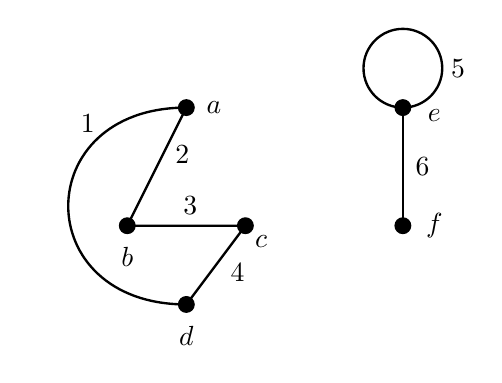
\begin{tikzpicture}
	\draw[line width=0.03cm] (0.75,-1) -- (1.5,0) -- (0,0) -- (0.75,1.5);
	\draw[line width=0.03cm] (0.75,1.5) to[bend right=90, distance=2cm] (0.75,-1);
	
	\draw[line width=0.03cm] (3.5,0) -- (3.5,1.5);
	\draw[line width=0.03cm] (3.5,2) circle (0.5);
	
	\draw[fill=black] (0,0) circle (0.1); 
	\draw[fill=black] (1.5,0) circle (0.1); 
	\draw[fill=black] (0.75,1.5) circle (0.1); 
	\draw[fill=black] (0.75,-1) circle (0.1); 
	
	\draw[fill=black] (3.5,0) circle (0.1); 
	\draw[fill=black] (3.5,1.5) circle (0.1); 
	
	\node at (1.1,1.5) {$a$};
	\node at (0,-0.4) {$b$};
	\node at (1.7,-0.2) {$c$};
	\node at (0.75,-1.4) {$d$};
	\node at (3.9,1.4) {$e$};
	\node at (3.9,0) {$f$};
	
	\node at (-0.5,1.3) {$1$};
	\node at (0.7,0.9) {$2$};
	\node at (0.8,0.25) {$3$};
	\node at (1.4,-0.6) {$4$};
	\node at (4.2,2) {$5$};
	\node at (3.75,0.75) {$6$};
	\end{tikzpicture}
	\]

\begin{enumerate}[(a)]
\item What is adjacent to $a$?
\item What is adjacent to 3?
\item Are there parallel edges? Explain.
\item Is the graph connected? Explain.
\item Is the graph simple? Explain. 
\end{enumerate}



% Question 7
\newpage
\question[10]  Let $G$ be the graph given below:
	\[
	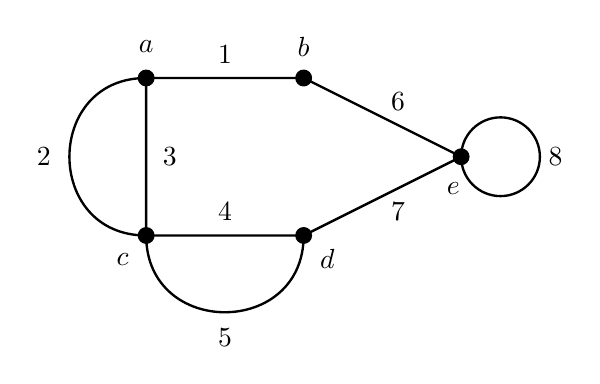
\begin{tikzpicture}
	\draw[line width=0.03cm] (4,1) -- (2,0) -- (0,0) -- (0,2) -- (2,2) -- (4,1);
	\draw[line width=0.03cm] (0,0) to[bend left=90, distance=1.3cm] (0,2);
	\draw[line width=0.03cm] (0,0) to[bend right=90, distance=1.3cm] (2,0);
	\draw[line width=0.03cm] (4.5,1) circle (0.5);
	
	\draw[fill=black] (0,0) circle (0.1);
	\draw[fill=black] (0,2) circle (0.1);
	\draw[fill=black] (2,2) circle (0.1);
	\draw[fill=black] (2,0) circle (0.1);
	\draw[fill=black] (4,1) circle (0.1);
	
	\node at (1,2.3) {$1$};
	\node at (-1.3,1) {$2$};
	\node at (0.3,1) {$3$};
	\node at (1,0.3) {$4$};
	\node at (1,-1.3) {$5$};
	\node at (3.2,1.7) {$6$};
	\node at (3.2,0.3) {$7$};
	\node at (5.2,1) {$8$};
	
	\node at (0,2.4) {$a$};
	\node at (2,2.4) {$b$};
	\node at (-0.3,-0.3) {$c$};
	\node at (2.3,-0.3) {$d$};
	\node at (3.9,0.6) {$e$};
	\end{tikzpicture}
	\]

\begin{enumerate}[(a)]
\item Find the degree of the vertex $c$.
\item Find the degree of the vertex $e$. 
\item Find the degree of the graph. 
\item Give an example of a trail from $a$ to $c$ that is not a path. 
\end{enumerate}



% Question 8
\newpage
\question[10]  Consider the graph below:
	\[
	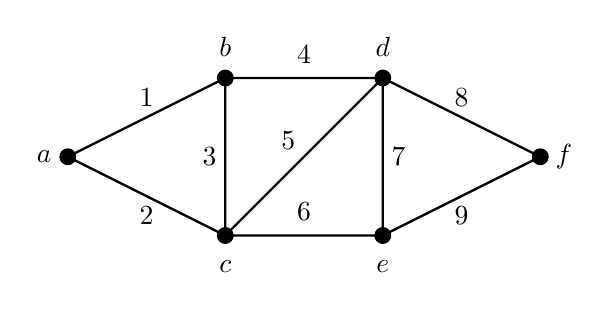
\begin{tikzpicture}
	\draw[line width=0.03cm] (0,2) -- (-2,1) -- (0,0);
	\draw[line width=0.03cm] (2,2) -- (0,2) -- (0,0) -- (2,0) -- (4,1) -- (2,2) -- (2,0);
	\draw[line width=0.03cm] (0,0) -- (2,2);
	
	\draw[fill=black] (-2,1) circle (0.1);
	\draw[fill=black] (0,0) circle (0.1);
	\draw[fill=black] (0,2) circle (0.1);
	\draw[fill=black] (2,0) circle (0.1);
	\draw[fill=black] (2,2) circle (0.1);
	\draw[fill=black] (4,1) circle (0.1);
	
	\node at (-2.3,1) {$a$};
	\node at (0,2.4) {$b$};
	\node at (0,-0.4) {$c$};
	\node at (2,2.4) {$d$};
	\node at (2,-0.4) {$e$};
	\node at (4.3,1) {$f$};
	
	\node at (-1,1.75) {$1$};
	\node at (-1,0.25) {$2$};
	\node at (-0.2,1) {$3$};
	\node at (1,2.3) {$4$};
	\node at (0.8,1.2) {$5$};
	\node at (1,0.3) {$6$};
	\node at (2.2,1) {$7$};
	\node at (3,1.75) {$8$};
	\node at (3,0.25) {$9$};
	\end{tikzpicture}
	\]

\begin{enumerate}[(a)]
\item Explain why the graph does not have an Euler circuit. 
\item Explain why the graph has an Euler trail. 
\item Find an Euler trial for this graph. 
\end{enumerate}



% Question 9
\newpage
\question[10] Consider the graph below:
	\[
	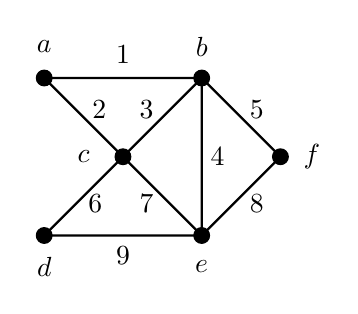
\begin{tikzpicture}
	\draw[line width=0.03cm] (2,2) -- (3,1) -- (2,0) -- (2,2) -- (0,2) -- (1,1) -- (0,0) -- (2,0) -- (1,1) -- (2,2);
	
	\draw[fill=black] (0,0) circle (0.1);
	\draw[fill=black] (2,0) circle (0.1);
	\draw[fill=black] (0,2) circle (0.1);
	\draw[fill=black] (2,2) circle (0.1);
	\draw[fill=black] (1,1) circle (0.1);
	\draw[fill=black] (3,1) circle (0.1);
	
	\node at (0,2.4) {$a$};
	\node at (2,2.4) {$b$};
	\node at (0.5,1) {$c$};
	\node at (0,-0.4) {$d$};
	\node at (2,-0.4) {$e$};
	\node at (3.4,1) {$f$};
	
	\node at (1,2.3) {$1$};
	\node at (0.7,1.6) {$2$};
	\node at (1.3,1.6) {$3$};
	\node at (2.2,1) {$4$};
	\node at (2.7,1.6) {$5$};
	\node at (0.65,0.4) {$6$};
	\node at (1.3,0.4) {$7$};
	\node at (2.7,0.4) {$8$};
	\node at (1,-0.25) {$9$};
	\end{tikzpicture}
	\]

\begin{enumerate}[(a)]
\item Find an Euler circuit for this graph. 
\item Find a Hamiltonian circuit for this graph. 
\end{enumerate}



% Question 10 
\newpage
\question[10] Let $G$ be the graph below:
	\[
	\begin{tikzpicture}
	\begin{scope}[very thick,decoration={
	markings,
	mark=at position 0.5 with {\arrow{>}}
				}
	] 
	
	\draw[line width=0.03cm,postaction={decorate}] (0,0) -- (2.5,0);
	\draw[line width=0.03cm,postaction={decorate}] (0,0) -- (1.25,2);
	\draw[line width=0.03cm,postaction={decorate}] (1.25,2) -- (2.5,0);
	\draw[line width=0.03cm,postaction={decorate}] (0,0) to[out= -30,in= -150] (2.5,0);
	\draw[line width=0.03cm,postaction={decorate}] (0,0) to[out= 30,in= 150] (2.5,0);
	\draw[line width=0.03cm,postaction={decorate}] (1.25,2) to[out= -30,in= 90] (2.5,0);
	\draw[line width=0.03cm,postaction={decorate},domain= 420:60] plot ({-0.33+0.433*cos(\x)}, {-0.33+0.433*sin(\x)});
	\draw[line width=0.03cm,postaction={decorate},domain= 120:480] plot ({2.83+0.433*cos(\x)}, {-0.33+0.433*sin(\x)});

	\draw[fill=black] (0,0) circle (0.1);
	\draw[fill=black] (2.5,0) circle (0.1);
	\draw[fill=black] (1.25,2) circle (0.1);
	\end{scope}
	\end{tikzpicture}
	\]

\begin{enumerate}[(a)]
\item Find the adjacency matrix for $G$.
\item Find the number of walks from 1 to 3 of length 2. 
\end{enumerate}


\end{questions}
\end{document}